\documentclass[letter,10pt,oneside]{article}
 
\usepackage{amsfonts}
\usepackage{amsmath}
\DeclareMathOperator*{\amax}{arg\,max}
\DeclareMathOperator*{\amin}{arg\,min}
\usepackage{amssymb}
\usepackage{dsfont}

\usepackage{epsf}
\usepackage{epsfig}
\usepackage{graphicx}
%\usepackage{wrapfig}
%\usepackage{subfig}

\usepackage{setspace}
\usepackage{geometry}
\usepackage{fancyhdr}

\usepackage{hyperref}
\hypersetup{
    colorlinks,
    citecolor=blue,
    filecolor=blue,
    linkcolor=blue,
    urlcolor=blue
}

\usepackage[latin2]{inputenc}
\usepackage{lmodern} % ez eltu"nteti a raszteressget s mg jk is a betu"k
\usepackage{t1enc}


\usepackage[usenames]{color}
%\usepackage[colorlinks]{hyperref}
%\usepackage{showkeys}

%\onehalfspacing
\usepackage{indentfirst}
%\frenchspacing

\usepackage{listings}
\definecolor{mygreen}{rgb}{0,0.6,0}
\definecolor{mygray}{rgb}{0.5,0.5,0.5}
\definecolor{mymauve}{rgb}{0.58,0,0.82}

\lstset{ %
  backgroundcolor=\color{white},   % choose the background color; you must add \usepackage{color} or \usepackage{xcolor}; should come as last argument
  basicstyle=\footnotesize,        % the size of the fonts that are used for the code
  breakatwhitespace=false,         % sets if automatic breaks should only happen at whitespace
  breaklines=true,                 % sets automatic line breaking
  captionpos=b,                    % sets the caption-position to bottom
  commentstyle=\color{mygreen},    % comment style
  deletekeywords={...},            % if you want to delete keywords from the given language
  escapeinside={\%*}{*)},          % if you want to add LaTeX within your code
  extendedchars=true,              % lets you use non-ASCII characters; for 8-bits encodings only, does not work with UTF-8
  frame=single,	                   % adds a frame around the code
  keepspaces=true,                 % keeps spaces in text, useful for keeping indentation of code (possibly needs columns=flexible)
  keywordstyle=\color{blue},       % keyword style
  language=python,                 % the language of the code
  morekeywords={*,...},           % if you want to add more keywords to the set
  numbers=left,                    % where to put the line-numbers; possible values are (none, left, right)
  numbersep=5pt,                   % how far the line-numbers are from the code
  numberstyle=\tiny\color{mygray}, % the style that is used for the line-numbers
  rulecolor=\color{black},         % if not set, the frame-color may be changed on line-breaks within not-black text (e.g. comments (green here))
  showspaces=false,                % show spaces everywhere adding particular underscores; it overrides 'showstringspaces'
  showstringspaces=false,          % underline spaces within strings only
  showtabs=false,                  % show tabs within strings adding particular underscores
  stepnumber=1,                    % the step between two line-numbers. If it's 1, each line will be numbered
  stringstyle=\color{mymauve},     % string literal style
  tabsize=4,	                   % sets default tabsize to 2 spaces
  title=\lstname                   % show the filename of files included with \lstinputlisting; also try caption instead of title
}

\geometry{left=2.5cm,right=2.5cm,top=3.0cm,bottom=2.5cm}

\pagestyle{fancy}
\lhead{ }
\chead{ }
\rhead{\thepage}

\lfoot{ }
\cfoot{ }
\rfoot{P\'{e}ter K\'{o}m\'{a}r, Totient Inc., 2019}


\renewcommand{\headrulewidth}{0.4pt}
\renewcommand{\footrulewidth}{0.0pt}

\newcommand{\bel}{\begin{equation}}
\newcommand{\eel}{\end{equation}}
\newcommand{\be}{\begin{equation*}}
\newcommand{\ee}{\end{equation*}}

\newcommand{\bal}{\begin{eqnarray}}
\newcommand{\eal}{\end{eqnarray}}
\newcommand{\ba}{\begin{eqnarray*}}
\newcommand{\ea}{\end{eqnarray*}}

\newcommand{\ket}[1]{| #1 \rangle}
\newcommand{\Ket}[1]{\left| #1 \right\rangle}
\newcommand{\bra}[1]{\langle #1 |}
\newcommand{\Bra}[1]{\left\langle #1 \right|}

\newcommand{\no}{\noindent}

\newcommand{\ev}[1]{\langle #1 \rangle}
\newcommand{\Ev}[1]{\left\langle #1 \right\rangle}
\newcommand{\+}{^\dagger}
\newcommand{\s}{^\ast}
\newcommand{\T}{^\top}
\newcommand{\LL}{\mathcal{L}}
\newcommand{\PP}{\mathcal{P}}

\newcommand{\low}{\text{low}}
\newcommand{\high}{\text{high}}
\newcommand{\MLE}{\text{MLE}}

\newcommand{\refeq}[1]{Eq. \ref{#1}}
\newcommand{\reffig}[1]{Fig. \ref{#1}}

\newcommand{\blue}[1]{{\color{blue} #1}}


%\numberwithin{equation}{section}
%\numberwithin{figure}{section}
%\numberwithin{table}{section}

\author{P\'{e}ter K\'{o}m\'{a}r (Totient Inc.)}
\title{Improved Fast Bayesian Matching Pursuit Algorithm}
\date{\today}


\begin{document}


\thispagestyle{empty}
\maketitle

\no {\bf One sentence summary: } We develop the mathematical formulas for an improved version of the FBMP algorithm and fine tune the algorithm for robust feature selection.

\section*{Summary}
Fast Bayesian Matching Pursuit (FBMP) is an algorithm published in 2008 by Schniter et al., designed to solve the sparse linear regression problem. In this problem, there are fewer samples than features, which renders the common strategies (such as OLS, Pursuit) for fitting a linear model useless. The main challenge of the sparse problem is to select which features are active, i.e. have non-zero coefficients.

The key idea of FBMP is to rely on the Bayesian model evidence as the primary metric for comparing  different sets of features. This metric can be efficiently calculated on a path of models, where consecutive models differ by the inclusion/exclusion of exactly one feature. Averaging the predictions of different plausible models yields a robust estimate of the linear coefficients.

The main difficulty that FBMP faces is the optimization of three hyperparameters ($\lambda, \sigma_x, \sigma$), which have significant effect on the set of active features in the final result. The expectation maximization scheme presented in their paper allows one to find the optimal values of these hyperparameters, but since these are point estimates, this strategy results in overfitting in terms of the set of active features.

Here we improve upon the methods of FBMP by
\begin{itemize}
  \item Requiring that the input features and targets are normalized, which allows us to define a proper prior for $\sigma_x$ and average over it.
  \item Assuming a proper prior for $\lambda$ and average over it.
  \item Repeating the model discovery process for a range of $\alpha = \sigma / \sigma_x$ values, and estimating their ``empirical prior'', which we then use to average over the models.
  \item Recording the immediate environment of the discovered path of models, which requires no extra computational time, only space.
  \item Avoiding computing the mean and covariance of linear coefficients, since they are irrelevant in determining which features are active.
  \item Instead of repeating the model search multiple times, we carry out a band search, which avoids re-computing the evidence already discovered models.
  \item We perform this band search in a way that ensures that all features are investigated.
\end{itemize}


\newpage
\tableofcontents

\newpage

\section{Input data}

Identically to the setup of linear regression, we assume that our data consist of $M$ samples $m\in \{1,2, \ldots M\}$, for which we record the values of 
\begin{itemize}
  \item $A = \big[[a_{m,n}]_{n=1}^N\big]_{m=1}^M \in \mathds{R}^{M\times N}$ features (assumed to be normalized such that $\sum_m a_{m,n} = 0$ and $\sum_m a_{m,n}^2 = M$, $\forall n$), and
  \item $y = [y_m]_{m=1}^M \in \mathds{R}^{M}$ targets (assumed to be normalized such that $\sum_m y_m = 0$ and $\sum_m y_m^2 = M$).
\end{itemize}

\section{Model}

\subsection{Bernoulli-Gaussian linear model}
The linear model dictates that $\mathbb{E}(y) = Ax$, where $x = [x_n]_{n=1}^N\in\mathds{R}^N$ are unknown linear coefficients. We assume uncorrelated Gaussian noise with uniform strength ($\sigma$) on all samples, allowing us to write the likelihood as a multivariate normal distribution,
\be
  P(y\;|\;x, \sigma) = \text{Normal}(y\;|\;Ax, \sigma^2 I_M),
\ee
where $I_M$ is the $M\times M$ identity matrix.
For the coefficients $x$, we adopt the Bernoulli-Gaussian model, where binary variables $s = [s_n]_{n=1}^N\in\{0,1\}^N$ indicate whether the corresponding $x$ values are non-zero, and $\sigma_x$ sets the typical scale of the non-zero coefficients:
\ba
  P(x\;|\;s, \sigma_x) = \left[\prod_{n: s_n = 0}\delta(x_n)\right] \times \left[\prod_{n: s_n=1} \text{Normal}(x_n\;|\;0, \sigma_x^2)\right],
\ea
where delta-functions ($\delta$) serve as the ``spike'', and the normal distribution as the ``slab'', from the ``spike and slab'' terminology. This model is depicted in \reffig{fig:summary}.
\begin{figure}[h]
  \centering
  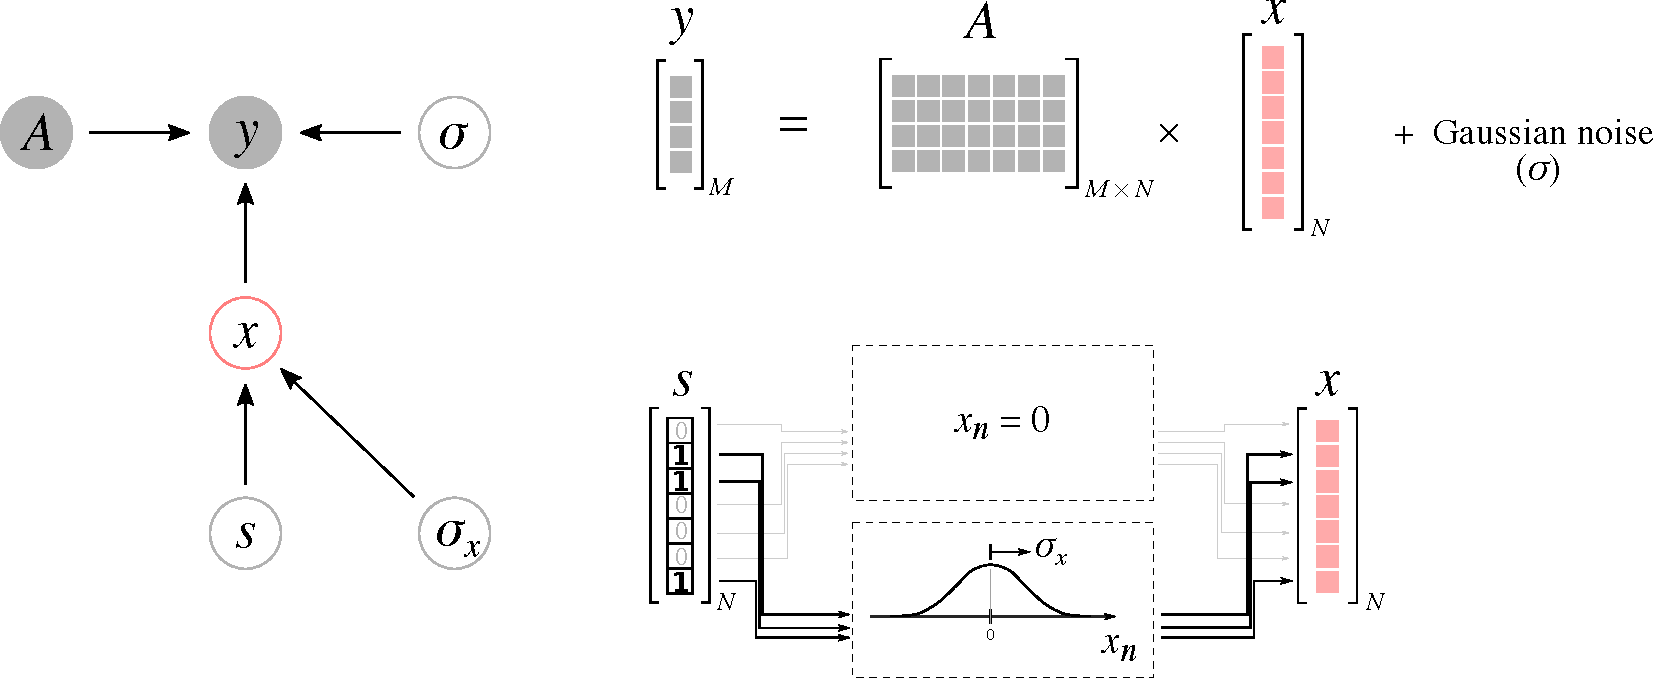
\includegraphics[width=0.9\textwidth]{figs/model-summary.pdf}
  \caption{
    \label{fig:summary}
    Summary of the Bernoulli-Gaussian linear model. The observed target vector $y$ depends linearly on the known set of feature matrix $A$ and the unknown coefficient vector $x$. These coefficients are assumed to be generated by the Bernoulli-Gaussian process, where the coefficient for the $n$th feature $x_n = 0$ ($\neq 0$) if $s_n = 0$ ($=1$), and the non-zero coefficients come from a zero-centered normal distribution with variance $\sigma_x^2$.}
\end{figure}

We denote the prior probability of any one feature being active by $\lambda$,
\be
  P(s\,|\,\lambda) = (1- \lambda)^{N_0(s)}\; \lambda^{N_1(s)}, \quad\text{where}\quad N_1(s) = N - N_0(s) = \sum_n s_n.
\ee
The hyperparameter $\lambda$ controls the number of non-zero elements of $s$. To enable inference with both strictly and loosely defined $\lambda$ values, we assume a beta prior for $\lambda$:
\be
  P(\lambda) = \text{Beta}(\lambda\,|\,a = \kappa \pi, b = \kappa (1-\pi)),
\ee
where $\pi$ and $\kappa$ control of the expectation value and the concentration of $\lambda$. With this choice the prior on $s$ is
\be
  p_s := P(s) = \intop\! d\lambda\, P(s\,|\,\lambda) P(\lambda) = \frac{\Gamma(\kappa)}{\Gamma(\kappa\pi)\Gamma(\kappa(1-\pi))} \frac{\Gamma\Big(\kappa \pi + N_1(s)\Big) \, \Gamma\Big(\kappa(1-\pi) + N_0(s)\Big)}{\Gamma\Big(\kappa + N\Big)},
\ee
and the number of active features is distributed, a priori, as a Beta-Binomial variable,
\be
  P(N_1 = K) = \sum_{s:N_1(s) = K} P(s) \;=\; {N \choose K} \,P(\text{any } s\,:\,N_1(s) = K) =  \text{BetaBinomial}(K\;|\; N, a = \kappa \pi, b = \kappa (1 - \pi)).
\ee


\subsection{Model evidence of $s$}
For any given $s$ vector, $P(x\;|\;s, \sigma_x)$ is a normal distribution with covariance $\sigma_x^2 D_s$, where $D_s = \text{diag}(s)$ is an $N\times N$ diagonal matrix where the diagonal is made of the components of $s$. The target $y$, being the linear combination of $x$ and the Gaussian noise, is also normally distributed with covariance $\sigma_x^2 A D_s A\T + \sigma^2 I_M$:
\be
  P(y\;|\;s, \sigma_x, \sigma) = \text{Normal}(y\;|\; 0, \;\sigma_x^2 A D_s A\T + \sigma^2 I_M),
\ee
yielding the model log likelihood in a closed form,
\bel
\label{eq:nu}
  \ln P(y\,|\,s, \sigma_x, \alpha) = -\frac{1}{2\sigma_x^2} y\T [\Phi(s, \alpha)]^{-1} y - \frac{M}{2}\ln(2\pi \sigma_x^2) - \frac{1}{2}\ln \det(\Phi(s,\alpha)),
\eel
where we defined $\alpha := \sigma / \sigma_x$ (representing the noise strength relative to the size of the linear coefficients), and
\be
  \Phi(s, \alpha) := A D_s A\T + \alpha^2 I_M \in \mathds{R}^{M\times M}.
\ee

To eliminate the dependence of \refeq{eq:nu} from $\sigma_x$, we assume an inverse-gamma prior for $\sigma_x^2$,
\be
  \ln P(\sigma_x^2) = \ln\left(\text{InvGamma}(\sigma_x^2\;|\;a, b)\right) = -(1 + a) \ln(\sigma_x^2) - \frac{b}{\sigma_x^2}.
\ee
Choosing $a = 1$ and $b = 1$ is identical to assuming that $1/\sigma_x^2$ is exponentially distributed with mean 1. This choice can be motivated by the maximum entropy principle and the fact that, after $y$ and columns of $A$ are normalized we expect $\sigma_x$ to be in the order of magnitude of 1. Alternatively, one may choose $a = 0$, $b = 0$, resulting in a scale-invariant (and improper) prior $P(\sigma_x^2) \propto \frac{1}{\sigma_x^2}$.

This choice of prior allows us to integrate out $\sigma_x$ from \refeq{eq:nu}, and obtain the formula for model evidence of $s$ that depends only on $\alpha$:
\bel
\label{eq:evidence}
  \ln P(y\,|\, s, \alpha) = \underbrace{-\frac{1}{2}\ln\det(\Phi(s,\alpha)) - \left(\frac{M}{2} + a\right)\ln\left(b + \frac{1}{2}y\T [\Phi(s,\alpha)]^{-1} y\right)}_{=:\, \ln L(s, \alpha)} \;+\; \text{const.}
\eel
where const. represents terms independent of $s$ or $\alpha$.


\subsection{Posterior}
\label{sec:posterior}
Our main focus is to obtain posterior probabilities for $s$, and the marginal of its elements $s_n$, and $N_1(s)$,
\ba
  p_n := P(s_n = 1\,|\, y) &=& \sum_{s: s_n = 1} P(s\,|\, y),\qquad \text{for all }n = 1,2\ldots N,\qquad \text{and} \\
  P(N_1(s) = K\,|\, y) &=& \sum_{s: N_1(s) = K} P(s\,|\, y),\qquad \text{for all }K = 0, 1,2\ldots N
\ea
Using the prior $p_s = P(s)$ allows us to write
\be
  P(y,s|\,\alpha) = p_s\,P(y\,|\,s, \alpha) \propto p_s\,L(s,\alpha) \quad \text{ and } \quad 
  P(s\,|\,y, \alpha) = \frac{P(y,s\,|\,\alpha)}{P(y\,|\,\alpha)} = \frac{p_s\,L(s, \alpha)}{\sum_{s'} p_{s'}\,L(s', \alpha)}
\ee
To eliminate $\alpha$, we use an empirical Bayes strategy: 

\begin{enumerate} 
  \item We estimate the posterior of $\alpha$,
  \be
    P(\alpha\,|\,y) = \frac{P(y\,|\,\alpha)P(\alpha)}{\intop\! d\alpha'P(y\,|\,\alpha')P(\alpha')} \approx \frac{P(y\;|\;\alpha)}{\sum_{\alpha'\in\mathcal{A}}P(y\;|\;\alpha')} = \frac{\sum_{s'} p_{s'}L(s', \alpha)}{\sum_{\alpha'\in\mathcal{A}}\sum_{s'} p_{s'}L(s', \alpha')} =: Q_\alpha,
  \ee
  where $\mathcal{A}$ is a finite set of discrete $\alpha$ values that we treat as a piori equiprobable. (For this, we will use a uniform grid on log-scale).

  \item Second, we use it as a prior for estimating model evidence,
  \be
    P(\alpha) \leftarrow P(\alpha\,|\,y) \approx \sum_{a\in \mathcal{A}} Q_a \delta(\alpha - a),
  \ee
  leading to
  \bel
    P(s\,|\,y) = \frac{P(y, s)}{P(y)} = \frac{\intop\! d \alpha\, p_s L(s, \alpha)\,P(\alpha)}{\sum_{s'}\intop\! d \alpha\, p_{s'} L(s', \alpha)\,P(\alpha)} \approx \frac{\sum_{\alpha \in \mathcal{A}} p_s L(s, \alpha) \,Q_\alpha}{\sum_{s'}\sum_{\alpha \in \mathcal{A}} p_{s'} L(s', \alpha) \,Q_\alpha},
  \eel
  and the marginals,
  \bal
    p_n = P(s_n = 1\,|\,y) &\approx & \frac{\sum_{\alpha \in \mathcal{A}} Q_\alpha \sum_{s:s_n=1} p_s L(s, \alpha)}{\sum_{\alpha \in \mathcal{A}} Q_\alpha \sum_{s'}p_{s'}L(s', \alpha)} \\
    P(N_1(s) = K\,|\,y) &\approx & \frac{\sum_{\alpha \in \mathcal{A}} Q_\alpha \sum_{s:N_1(s)=K} p_s L(s, \alpha)}{\sum_{\alpha \in \mathcal{A}} Q_\alpha \sum_{s'}p_{s'}L(s', \alpha)}
  \eal

\end{enumerate}

Note: While using $Q_\alpha$ in place of the prior $P(\alpha)$ in the final result can still result in overfitting, averaging over multiple plausible values of $\alpha$ makes this result more robust than the maximum likelihood estimate,
\be
  P(s\,|\,y,\alpha^\text{MLE}) = \frac{p_s L(s, \alpha^\text{MLE})}{\sum_{s'} p_{s'}L(s', \alpha^\text{MLE})},\qquad \text{where }\quad \alpha^\text{MLE} = \amax_\alpha \sum_{s'}p_{s'}L(s', \alpha).
\ee

\subsection{Estimation of coefficients}
We can compute the posterior mean of the linear coefficients $x$,
\be
  x_\text{mmse} := \mathbb{E}(x\;|\;y) = \sum_s P(s\;|\;\alpha, y) P(\alpha) \mathbb{E}(x\;|\;s, \alpha, y) \approx \frac{\sum_s \sum_\alpha p_{s} L(s, \alpha) Q_\alpha \mathbb{E}(x\;|\;s, \alpha, y)}{\sum_s \sum_\alpha p_{s} L(s, \alpha) Q_\alpha},
\ee
where the conditional expectation value can be computed in closed form
\ba
  \mathbb{E}(x\;|\;s, \alpha, y) &=& D_s A\T \big[\Phi(s, \alpha)\big]^{-1} y 
  = D_s A\T\big[AD_s A\T + \alpha^2 I_M\big]^{-1}y \\
  \mathbb{E}(x_s\;|\;s, \alpha, y) &=& \big[A_s\T A_s + \alpha^2 I_{N_1(s)}\big]^{-1}A_s\T y,
\ea
where, in the alternative formula, we use $A_s$ to denote the sub-matrix of $A$ consisting of the all columns $n$ for which $s_n = 1$, and $x_s$ is denotes the vector of non-zero elements of $x$.

\newpage
\section{Efficiently searching the model space}
\label{sec:Efficient_search}
With the formulas derived in the previous section, the inference task is reduced to evaluating $p_s$ and $L(s,\alpha)$ at all plausible models, $s\in \{0,1\}^N$. Unfortunately, this quickly becomes infeasible with increasing number of features $N$. We follow the strategy of the original FBMP, approximate the sums over $s$ with a partial sum, which we construct using a heuristic discovery algorithm that aims to find the $s$ models with the largest $p_s L(s, \alpha)$ contributions.

\subsection{Update formulas based on $\Phi$ matrix}
Since $p_s$ depends only on $N_1(s)$, we can pre-compute it for all $N_1(s) = 0, 1, 2, \ldots N$, and use it whenever needed. The real difficulty is posed by the computation of $L(s, \alpha)$, which requires calculating the determinant and the inverse of $\Phi(s,\alpha)$, an $M\times M$ matrix, for every $s$. Fortunately, as spelled out by the original publication of FBMP, we can speed up these calculations by relying on recursion formulas based on the matrix determinant lemma and the matrix inversion lemma.

Let's assume that we already computed the following quantities for a model $s$
\ba
  G(s) &:=& \ln \det(\Phi(s)) \\
  H(s) &:=& y\T [\Phi(s)]^{-1} y \\
  c_k(s) &:=& [\Phi(s)]^{-1} a_k  \qquad \forall k = 1,2,\ldots N,
\ea
where $a_k$ is the $k$th column of $A$, and we dropped the $\alpha$ argument from $\Phi$ because it is assumed to be fixed throughout the entire search.

Now, we wish to evaluate $L(s')$, where $s'$ differs from $s$ only in the $n$th element, i.e. $s'_n = 1-s_n$, but $s'_k = s_k$ for all $k \neq n$. This changes $\Phi(s) \mapsto \Phi(s') = \Phi(s) + (-1)^{s_n}a_n a_n\T$. We can compute the effect of this change in the following ``discovery'' steps:
\bal
  \label{eq:beta_n}
  \beta_n(s) &:=& \left(1 + (-1)^{s_n} a_n\T c_n(s)\right)^{-1} \\
  \label{eq:Gnext_n}
  G^\text{next}_{n}(s) &:=& G(s) - \ln \beta_n(s) \\
  \label{eq:Hnext_n}
  H^\text{next}_{n}(s) &:=& H(s) - (-1)^{s_n}\beta_n(s) \left(c_n(s)\T y\right)^2 \\
  \ln L^\text{next}_n(s) &:=& -\frac{1}{2} G^\text{next}_{n}(s) - \left(\frac{M}{2} + a\right)\ln\left(b + \frac{H^\text{next}_{n}(s)}{2}\right) \\
  \ln L(s') &=& \ln L^\text{next}_n(s), \nonumber
\eal
where, to derive the formulas for $G^\text{next}$ and $H^\text{next}$, we used the matrix determinant and inversion lemmas in the following forms:
\ba
  \det \left(\Phi(s) + u_n a_n\T \right) &=& \Big(1 + a_n\T[\Phi(s)]^{-1} u_n \Big)\det (\Phi(s)) \\
  \Big[\Phi(s) + u_n a_n\T \Big]^{-1} &=& [\Phi(s)]^{-1} - [\Phi(s)]^{-1}u_n \Big(1 + a_n\T [\Phi(s)]^{-1}u_n\Big)^{-1}a_n\T [\Phi(s)]^{-1},
\ea
where $u_n = (-1)^{s_n} a_n$.
To proceed from the new state $s'$, we need to compute $G(s')$, $H(s')$ and $c_k(s')$. We refer to these as ``extension'' steps:
\bal
  G(s') &=& G_n^\text{next}(s) \nonumber\\
  H(s') &=& H_n^\text{next}(s) \nonumber\\
  c_k(s') &=& c_k(s) - (-1)^{s_n} \beta_n(s) c_n(s) \left(c_n(s)\T a_k\right).
\eal
These iteration steps are illustrated in \reffig{fig:iteration}.
\begin{figure}[h]
  \centering
  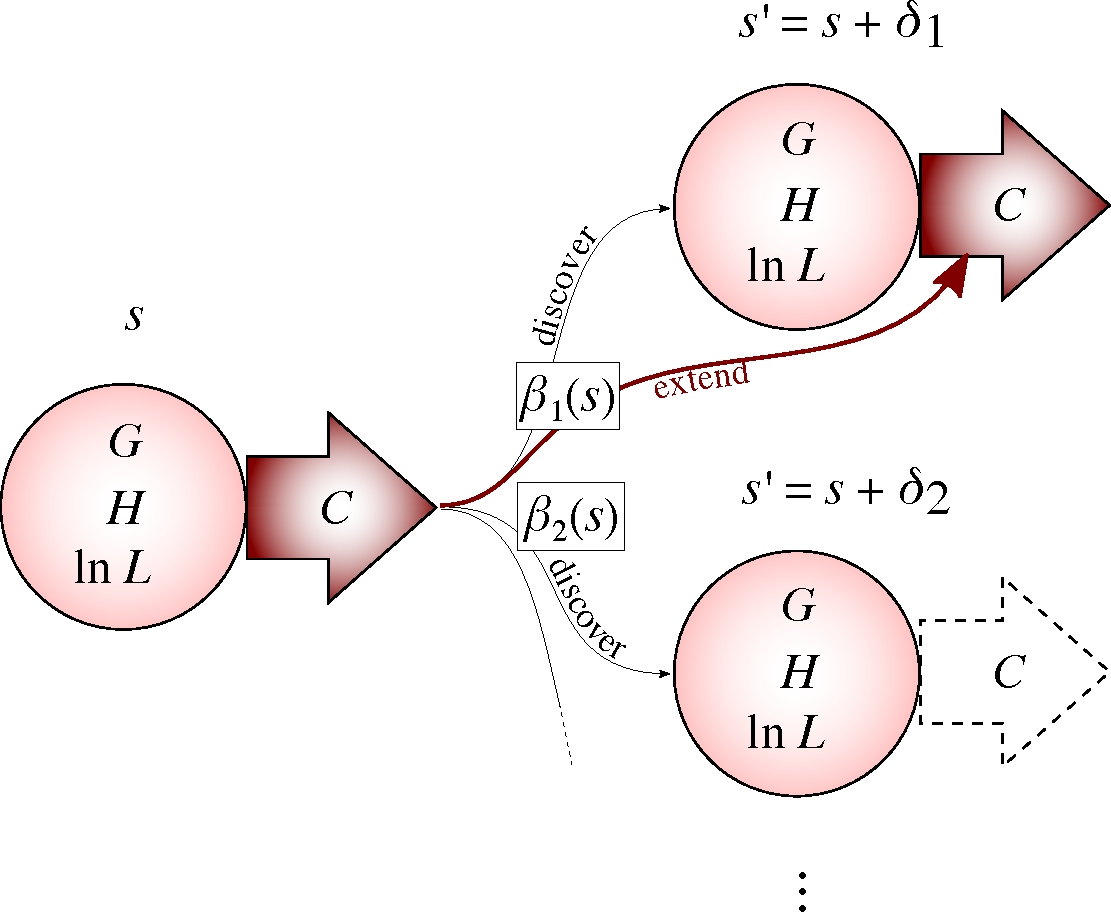
\includegraphics[width=0.4\textwidth]{figs/iteration.pdf}
  \caption{
    \label{fig:iteration}
    Discovery and Extension steps: {\bf Discovery:} We use $G(s), H(s)$ and $C(s)$ of the current state $s$ to compute the $G(s'), H(s'), \ln L(s')$ of all neighboring states $s'$. {\bf Extension:} From $C(s)$, we compute $C(s')$ for only a the selected $s'$ states that we decide to extend.
  }
\end{figure}

This closes the loop, and allows us to iteratively compute $\ln L$ on a sequence of models where consecutive  $s$ vectors differ in exactly one element by keeping track of $G(s), H(s)\in\mathds{R}$  and $C(s):=[c_k(s) ]_{k=1}^N \in \mathds{R}^{M\times N}$ in every step. 
The computational time is mostly spent on computing $2N$ dot products between $M$-vectors during discovery ($a_n\T c_n(s)$ and $c_n(s)\T y$, for all $n = 1, 2, \ldots N$), and $N$ dot products during extension ($c_{n\s}(s)\T a_k$ for all $k = 1, 2, \ldots N$). Therefore the time complexity is $\mathcal{O}(MN)$.


\subsection{Update formulas based on $\Psi$ matrix}
It is possible to improve on the time complexity of the update algorithm from $\mathcal{O}(MN)$ to $\mathcal{O}(N_1(s)N)$, where $N_1(s)$ is the number of \emph{active} features, i.e. $N_1(s) = \sum_{n} s_{n}$, which must be less than $M$ to avoid overfitting.

Instead of $\Phi(s) \in \mathds{R}^{M\times M}$, we are going to express $G(s)$ and $H(s)$ with the matrix $\Psi(s) \in \mathds{R}^{N_1(s)\times N_1(s)}$,
\ba
  \Psi(s) &:=& (A\T)_{s,:} A_{:,s} + \alpha^2 I_{N_1(s)} \\
  G(s) = \ln \det \Phi(s) &=& 2(M - N_1(s))\ln \alpha + \ln \det \Psi(s) \\
  H(s) = y\T [\Phi(s)]^{-1} y &=& \frac{1}{\alpha^2}\Big[y\T y - (y\T A_{:, s})[\Psi(s)]^{-1}((A\T)_{s,:} y)\Big] 
\ea
where the subscript $s$ represents selecting the rows (or columns) $n$ of the matrix corresponding to $s_n = 1$, and the placeholder ``$:$'' shows that all values of the index are used. For the expressions of $G$ and $H$, we used that $A D_s A\T = A_{:,s}(A\T)_{s,:}$ and the following matrix identities,
\be
  \det(I + AB\T) = \det(I + A\T B)
\ee
with ``$A$'' $=$ ``$B$'' $= \frac{1}{\alpha}A_{:,s}$, and
\be
  (A + BD^{-1}C)^{-1} = A^{-1} - A^{-1}B (D + CA^{-1}B)^{-1} C A^{-1}
\ee
with ``$A$'' $= \alpha^2 I_M$, ``$B$'' $= A_{:,s}$, ``$C$'' $= (A\T)_{s,:}$, and ``$D$'' $= I_P$.

We follow the same logic as the update equations in the previous subsection. Additionally, we introduce $\tilde s$, which contains the indexes of the ``1'' elements of $s$. The order of the elements of $\tilde s$ is defined, and reflects sequence of recursive updates that have been performed previously, therefore when used as an index, $\tilde s$ defines a particular order in which the rows or columns should be taken. We assume that we have already computed the following variables for a model $s$ (using the ordering $\tilde s$):
\ba
  z(\tilde s) &:=& [(A\T)_{\tilde s, :}]\,y \\
  B(\tilde s) &:=& (A\T A)_{\tilde s, :} \\
  G(s) &=& 2(M - P)\ln \alpha + \ln \det \Psi(s) \\
  H(s) &=& \frac{1}{\alpha^2}\Big[y\T y - [z(\tilde s)]\T[\Psi(\tilde s)]^{-1}z(\tilde s)\Big] \\
  c_n(\tilde s) &:=& [\Psi(\tilde s)]^{-1}[B(\tilde s)]_{:,n} \quad \in \mathds{R}^{N_1(s)} \qquad \text{for all } n = 1,2,\ldots N
\ea
With this, we can quickly compute $G(s')$ and $H(s')$ for all $s'$neighbors of $s$, for each of which only one element $s'_n$ is different, i.e. $s'_n = 1 - s_n$, but for all $k\neq n$, $s'_k = s_k$. In the case of $s_n = 0$, such a change from $s$ to $s'$ adds a new row and a new column to $\Psi(s)$, and it changes $\tilde s$ to $\tilde{s}' = [\tilde s, n]$:
\be
  \Psi(\tilde s) = \left[
  \begin{array}{ccc}
    & & \\
    & \Psi & \\
    & & 
  \end{array}
  \right] \in \mathds{R}^{N_1(s) \times N_1(s)}
  \quad \rightarrow \quad
  \Psi(\tilde{s}') = \left[
  \begin{array}{ccc|c}
    & & & \\
    & \Psi & & [B(\tilde s)]_{:,n}\\
    & & & \\
    \hline
    & ([B(\tilde s)]_{:,n})\T& & \alpha^2 + (A\T A)_{n,n}
  \end{array}
  \right] \in \mathds{R}^{(N_1(s) + 1) \times (N_1(s) + 1)}
\ee
We compute the effect of this change with the following formulas. This is the ``discovery'' step.
\bal
  \beta_n(s) &=& \Big(\alpha + (-1)^{s_n}\big[(A\T A)_{n,n} -  [B(\tilde s)]_{:,n})\T c_n(\tilde s)\big]\Big)^{-1} \\
  G^\text{next}_n(s) &=& G(s) - \ln (\alpha^2 \beta_n(s)) \\
  H^\text{next}_n(s) &=& H(s) - (-1)^{s_n} \frac{\beta_n(s)}{\alpha^2}\Big[[z(\tilde s)]\T c_n(\tilde s) - (A\T y)_n\Big]^2 \\
  \ln L^\text{next}_n(s) &:=& -\frac{1}{2} G^\text{next}_{n}(s) - \left(\frac{M}{2} + a\right)\ln\left(b + \frac{H^\text{next}_{n}(s)}{2}\right) \\
  \ln L(s') &=& \ln L^\text{next}_n(s), \nonumber
\eal
where, to derive the formulas for $G^\text{next}$ and $H^\text{next}$, we used the following identities for block matrices
\ba
  \det\left[
  \begin{array}{cc}
  A & b \\
  b\T & c
  \end{array}
  \right] 
  &=& 
  k \det(A),
  \\
  \left[
  \begin{array}{cc}
  A & b \\
  b\T & c
  \end{array}
  \right]^{-1} 
  &=&
  \left[
  \begin{array}{cc}
  A^{-1} + \frac{1}{k}A^{-1}bb\T A^{-1} & -\frac{1}{k}A^{-1}b \\
  -\frac{1}{k}b\T A^{-1} & \frac{1}{k}
  \end{array}
  \right],\\
  \text{where} \qquad k &=& c - b\T A^{-1}b.
\ea
with ``$A$'' $= \Psi$, ``$b$'' $=[B(\tilde s)]_{:,n}$, and ``$c$'' $=\alpha^2 + (A\T A)_{n,n}$.

Note: Using the above identities, only the $s_n=0$ cases of the discovery formulas can be proven. To get the $(-1)^{s_n}$ factors right, one needs to compare the results with equations Eqs. (\ref{eq:beta_n}) - (\ref{eq:Hnext_n}).

To proceed from the new $s'$ state, we need to compute $G(s')$, $H(s')$ and $z(\tilde{s}')$, $B(\tilde{s}')$, $c_k(\tilde{s}')\in \mathds{R}^{N_1(s) + 1}$ for all $k = 1,2,\ldots N$. This is the extension step:
\bal
  G(s') &=& G^\text{next}_n(s) \nonumber \\
  H(s') &=& H^\text{next}_n(s) \nonumber \\
  z(\tilde{s}') &=& \left[\begin{array}{c}
    \\
    z(\tilde s)\\
    \\
    \hline
    [A_{:,n}]\T y 
  \end{array}\right] \quad \in \mathds{R}^{N_1(s) + 1} \nonumber \\
  B(\tilde{s}') &=& \left[\begin{array}{ccc}
    & &  \\
    & B(\tilde{s}) & \\
    & & \\
    \hline
    & [A_{:,n}]\T A
  \end{array}\right] \quad \in \mathds{R}^{(N_1(s) + 1)\times N} \nonumber\\
  c_k(\tilde{s}') &=& 
  \left[\begin{array}{c}
    \\
    c_k(\tilde s) \\
    \\
    \hline
    0
  \end{array}\right] 
  + 
  \left[\begin{array}{c}
    \\
    c_n(\tilde s) \\
    \\
    \hline
    -1
  \end{array}\right] \beta_n(s)\Big([c_n(\tilde s)]\T [B(\tilde s)]_{:, k} - [B(\tilde{s}')]_{n,k}\Big) \quad \in \mathds{R}^{N_1(s)+1},
\eal
where the above update formula for $c_k(\tilde s) \rightarrow c_k(\tilde{s}')$ works only for adding features, i.e. when $s_n = 0$. The pursuit algorithm, which we describe next, uses only forward extensions, which means we do not need to compute the update formula for $c_k$ for the backward ($s_n = 1$) case.

Because the above formulas operate on vectors of length $N_1(s)$ (instead of length $M$), and most of the time is spent on $N$ dot products between such vectors, the time complexity is $\mathcal{O}(N_1(s) N)$, instead of $\mathcal{O}(MN)$. If we limit the depth of the pursuit to $N_{1,\text{max}}$, the total time will be $\mathcal{O}((N_{1,\text{max}})^2 N)$. Which, compared to the total runtime of the update equations that use $\Phi(s)$, $\mathcal{O}(N_{1,\text{max}} M N)$, suggests a speedup by a factor of $N_{1,\text{max}} / M$. With $M = 200$ samples, and $N_{1,\text{max}} = 20$ max depth, this is a 10-fold speedup. Furthermore, time complexity of the update formulas based on $\Psi$ is not increasing with the number of samples $M$. This is of great practical importance for applications where the amount of samples is expected to grow, but the plausible max number of active features remains constant.

Note: $A\T y$ and $\text{diag}(A\T A)$ need to be precomputed for an efficient algorithm. Since they are of length $N$, storing them is feasible. For small $N$, precomputing the entire $A\T A$ matrix may be feasible, but since it requires $\mathcal{O}(N^2)$ space, it is a better strategy to compute the required elements when they are needed. When $s$ changes to $s' = s + \delta_n$, the $(A\T A)_{n, :}$ vector need to be computed and stored alongside with the already computed $(A\T A)_{s, :}$ values. The required space grows as $\mathcal{O}(N_1(s) N)$, much less than $\mathcal{O}(N^2)$, because $N_1(s) < M < N$.

\subsection{Runtime comparison of update algorithms}
We run a simple benchmarking experiment to measure the running times of five different algorithms for computing $G(s)$ and $H(s)$ along a pre-defined path of model vectors:
\begin{enumerate}
  \item Using the definitions expressed with $\Phi(s)$
  \item Using the definitions expressed with $\Psi(s)$
  \item Recursive updates based on $\Phi(s)$
  \item Recursive updates based on $\Psi(s)$ (computing elements of $A\T A$ on the fly)
  \item Recursive updates based on $\Psi(s)$ (with precomputed $A\T A$)
\end{enumerate}
on \reffig{fig:runtimes}. This shows that recursive updates based on $\Psi$ are the fastest, as long as $N_1(s) < M/2$.

\begin{figure}[h]
  \centering
  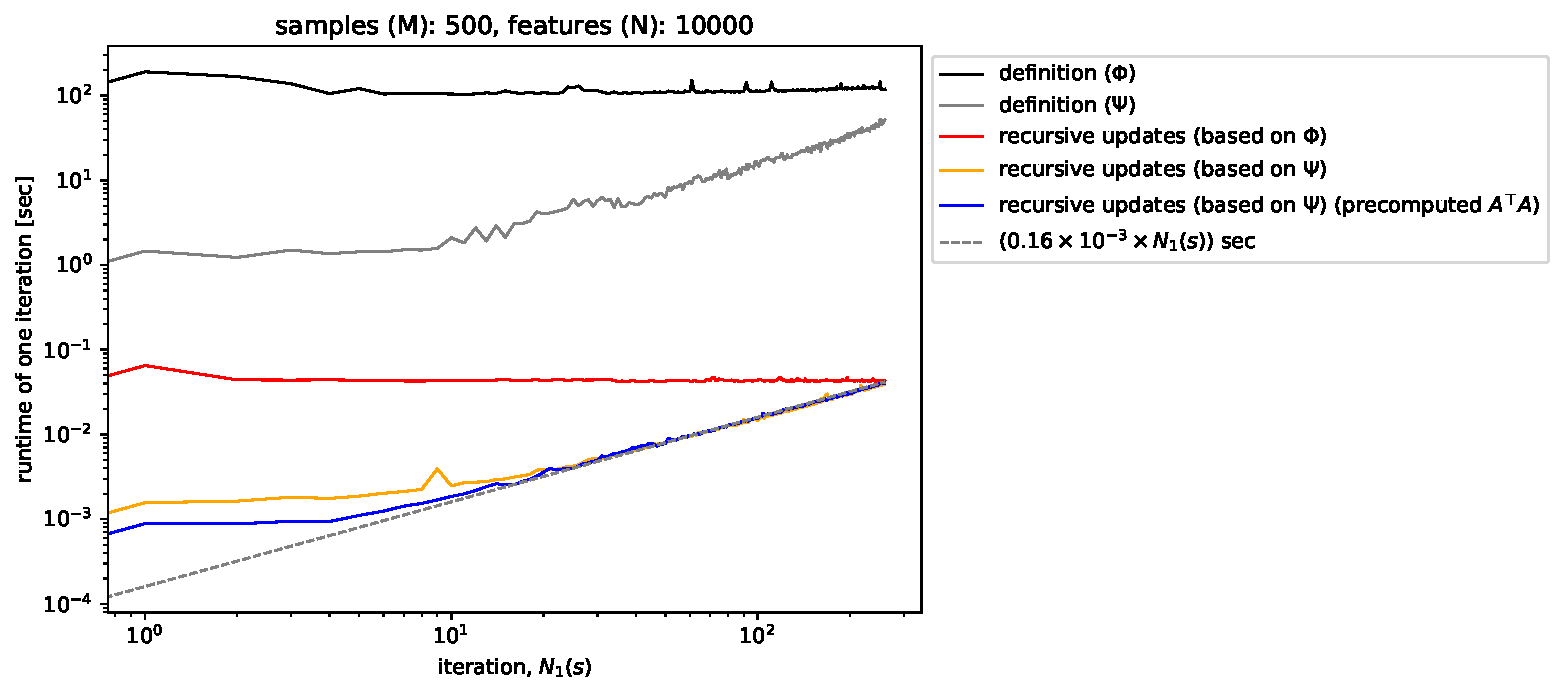
\includegraphics[width=\textwidth]{./figs/runtimes.pdf}
  \caption{
    \label{fig:runtimes}
    Comparison of running time required by each algorithm to compute $G$ and $H$ in the the immediate environment of any particular $s$ vector and move to the next $s$ vector on a pre-defined path. We used $M = 500$ samples and $N = 10,\!000$ features.
  }
\end{figure}

\subsection{Pursuit algorithm}
Using the update formulas $(G(s), H(s), C(s)) \mapsto (G(s'), H(s'), C(s'))$, where $C(s) = [c_1(s), c_2(s), \ldots c_N(s)]$, we can quickly compute $L$ on a pre-defined path in $s$-space. Since it is not feasible to compute $L$ on all $s$, we wish to find paths with high $L$. For this, we adopt the greedy search algorithm presented in the original publication of FBMP.
\begin{enumerate}
  \item Start from a particular state, $s_0$, and compute $G(s_0)$, $H(s_0)$ and $C(s_0)$, using their definitions.
  \item In state $s$, use the ``discovery'' formulas to compute $\ln L^\text{next}_n(s)$ for all $n=1,2,\ldots N$.
  \item Choose the best feature to add,
    \be
      n\s = \amax_{n: s_n = 0} \,\ln L^\text{next}_n(s),
    \ee
    or, if $N_1(s) = N_{1,\text{max}}$, break iteration. 
    Here the requirement of $s_n = 0$ ensures that we only consider adding a feature and not removing one. The threshold $N_{1,\text{max}} (\leq N)$ is used to terminate the search before it reaches the endpoint, i.e. $s=(1,1,\ldots 1)$.
  \item Construct $s'$ from $s$ by flipping its $n\s$th element to 1. 
  \item Using the ``extension'' formulas with $n\s$, compute $G(s'), H(s'), C(s')$, and return to step 2 with the new $s'$.
\end{enumerate}

While this algorithm is traversing the $s$-space, we can continually record all computed $\ln L(s') = \ln L^\text{next}_n(s)$ values and their corresponding states $s' = s + \delta_n \mod 2\;, \forall n = 1,2,\ldots N$, where $\delta_n$ is a binary vector where only the $n$th component is 1.


\subsection{Deploying}

\no To  get the most use out of the pursuit algorithm, we deploy it with the following details.

\begin{itemize}
  \item We start the pursuit from the null model, $s_0 = (0,0,\ldots 0)$.
\end{itemize}

Earlier, we expressed the formulas for ``discovery'' and ``extension'' in terms of change of single features $n$, but these equations can be vectorized to decrease computational time.
\begin{itemize}
  \item During each ``discovery'' step, we compute the vectors $\beta = [\beta_n]_{n=1}^N$, $G^\text{next} = [G^\text{next}_n]_{n=1}^N$ and $H^\text{next} = [H^\text{next}_n]_{n=1}^N$
  \item During each ``extension'' step, we compute the matrix $C = [c_k]_{k=1}^N$.
\end{itemize}

The pursuit strategy realizes a greedy search, which can miss the $s$ vectors with the highest model evidences. To increase our chances of discovering the most likely models, we perform a band search.

\begin{itemize}
  \item Instead of selecting one $n\s$ (and one $s'$) to move forward with, we select $B$ number of $s'$ models with the highest $\ln L(s')$ to extend in each step. Their extensions will result in a discovery of a larger set of $s$-vectors compared to the single-extension strategy. We call $B$ the ``bandwidth'' of the band search. This is illustrated for $B = 2$ in \reffig{fig:band_search}.
\end{itemize}
\begin{figure}[h]
  \centering
  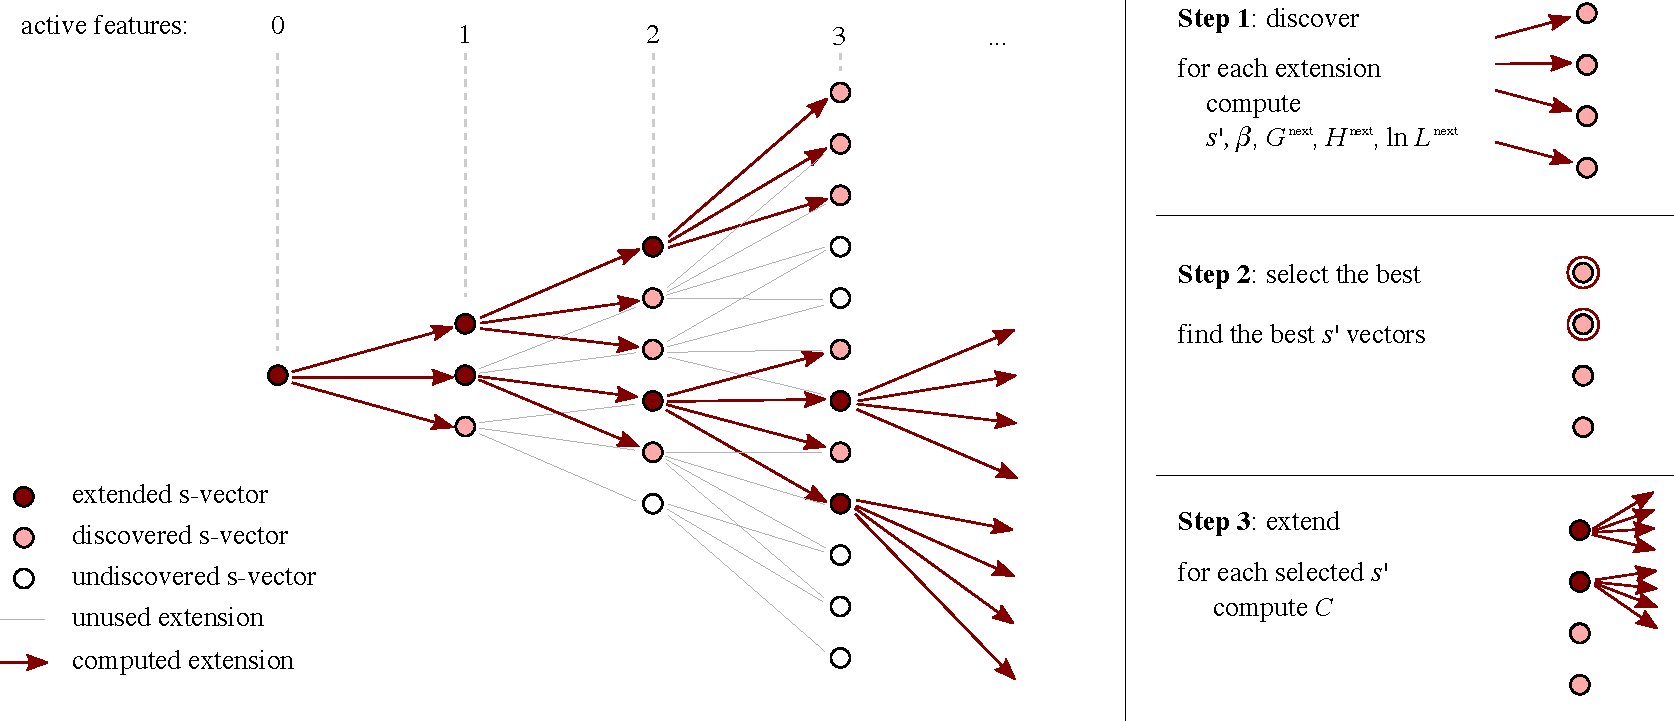
\includegraphics[width=\textwidth]{figs/extension.pdf}
  \caption{
    \label{fig:band_search}
    Band search: In each iteration of the band search, we first compute $\ln L(s')$ for all neighboring nodes of the extended nodes. Second, from among these newly discovered nodes, we select the $B$ best, i.e. with the highest $\ln L(s')$. Finally, we compute the $C$ matrix for each selected node, which allows us to extend these nodes in the next iteration.
  }
\end{figure}

A naive implementation of the band search would result in computing $\ln L(s')$ for the same $s'$ multiple times in a round of extensions whenever $s'$ can be reached from two different $s$ nodes that we are extending. 
\begin{itemize}
  \item To avoid this waste of computation, we keep track of the set of already discovered $s$ vectors, and perform the calculation of $\beta_n(s), G^\text{next}_n(s)$, $H^\text{next}_n(s)$ and $\ln L^\text{next}_n(s)$ only if the target node $s' = s + \delta_n$ has not been discovered before. (This is also illustrated on \reffig{fig:band_search} for the extensions between layer 1 and 2.)
\end{itemize}


It is known that sparse regression models are capable of discovering the relevant features only if there are more samples than active features. One can show this for FBMP by considering that, for small enough $\alpha$, we can approximate the $\Phi$ matrix as $\Phi(s, \alpha) \approx P_s A_s A_s\T P_s + \alpha^2(I_M - P_s)$, where $A_s = AD_s$ and $P_s = A_s(A_s\T A_s)^{-1} A_s\T$ is the projector to the subspace spanned by the eigenvectors of $A_sA_s\T$ with positive eigenvalues. When using this approximation in the formula for $P(y\,|\,s, \sigma_x, \alpha)$, the $\alpha$-dependent part gives rise to a factor of Gaussian pdf, $\text{Normal}((I_M - P_s)y\,|\,0,\, \sigma_x^2 \alpha^2 (I_M - P_s))$. This factor behaves differently depending on whether $(I_M - P_s)y$ is zero. Since $y$ is normalized it resides in an $M-1$ dimensional subspace of $I_M$, which may be fully covered by $P_s$ if its rank is at least $M-1$. By limiting our investigation to models where $N_1(s) \leq M - 2$, we can guarantee that the rank of $P_s$ is smaller than $M - 1$, and cannot cover this ``normalized subspace'' of $I_M$, and as a result $P(y\,|\,s, \sigma_x, \alpha)\rightarrow 0$ as $\alpha \rightarrow 0$, avoiding overfitting.
\begin{itemize}
  \item We stop all pursuits before reaching this boundary, i.e. we set $N_{1,\text{max}} = M - 2$.
\end{itemize}

Our main focus is estimating the marginals $p_n = P(s_n = 1\;|\;y)$, and we wish to avoid false positive results due to incomplete discovery of the $s$ space, i.e. cases where the approximated $p_n$ is much higher than what the full model would give if we could compute $L(s)$ for all $s$. The pursuit algorithm is designed to discover the most likely $s$ models (and their immediate neighbors). If a feature $n$ is favorable to be included, its indicator $s_n$ will be 1 for the vast majority of the states discovered by the pursuit. This results in undersampling the states where the feature is inactive, and overestimating the models confidence that this feature is active.
\begin{itemize}
  \item In each layer of the search, we investigate each feature to some extent, no matter how unfavorable it is to include them. We do this by extending a larger set of features in each layer, a set that we construct by making sure that both values (0 and 1) of every $s_n$ indicator are represented at least $B$ times. This construction is done step by step, where in each step we add the $s'$ vector with the highest $\ln L$ that increments any of the counters $\{|\{s\,:\, s_n=0\}|\}_{n=1}^N$ and $\{|\{s\,:\, s_n=1\}|\}_{n=1}^N$ that are still below $B$.
\end{itemize}

Discovering and recording many $(s, L(s))$ pairs can result in filling up computer memory. In cases where we are interested only in certain aggregate statistics about $P(s\;|\;y)$, we can discard intermediate results: it is enough to keep track of particular cumulative sums.
\begin{itemize}
  \item To estimate $Q_\alpha$, we only need the cumulative sum of $\sum_s p_s L(s, \alpha)$.
  \item To estimate $p_n$, we only need the cumulative sums of $\sum_{s: s_n =  1} p_s L(s, \alpha)$ and $\sum_{s: s_n=0} p_s L(s, \alpha)$.
  \item To estimate the posterior of $N_1$ (the number of active features), we only need the cumulative sum of $\sum_{s: N_1(s) = K} p_s L(s, \alpha)$ for every $K=0,1,2,\ldots N$.
\end{itemize}

For the posteriors, we need to sum over a set of $p_s L(s, \alpha)$ values that often span many orders of magnitudes. This can cause numerical instabilities. To avoid it, we use the ``logsumexp'' function for summations over $s$ and $\alpha$
\begin{itemize}
  \item $\ln\Big(\sum_s p_s L(s, \alpha)\Big) = \text{logsumexp}_s\Big(\ln p_s + \ln L(s, \alpha)\Big)$
  \item $\ln \Big(\sum_\alpha Q_\alpha p_s L(s,\alpha)\Big) = \text{logsumexp}_\alpha\Big(\ln Q_\alpha + \ln p_s + \ln L(s, \alpha)\Big)$
\end{itemize}

After computing $Q_\alpha$ and $p_s L(s,\alpha)$, we know which $\alpha$ value and which $s$ models have the highest evidence. This enables us to prioritize them during the computation of $x_\text{mmse}$. We rely on the assumption that in most cases the top models encompass the majority of the posterior probability, and compute the following approximation of $x_\text{mmse}$ for as set of top models that we select in a way to ensure that all features $n$ are represented (i.e. $s_n=1$) at least ten times among the selected $s$ vectors.
\begin{itemize}
  \item $x_\text{mmse} \approx \sum_s p_s L(s, \alpha\s) \big[A_s\T A_s + \tilde{\alpha}^2 I_{N_1(s)}\big]^{-1}A_s\T y$,
\end{itemize}
where $A_s = [A_{m,n}\,:\,s_n=1]$ is the sub-matrix of $A$, $\alpha\s$ is the mode of $Q_\alpha$, and $\tilde \alpha$ is the ``log-mean'' of $\alpha$, i.e. $\tilde{\alpha} = \exp(\sum_\alpha Q_\alpha \log(\alpha) / (\sum_\alpha Q_\alpha))$. Since $N_1(s)$ is usually small, computing the inverse 


\section{Extension: Fixed features}
One can imagine a setting where, we would like to fix some of the features to be active, indicating that we are certain that they have some non-zero effect. Here we extend the FBMP model to handle this setup.

\subsection{Input data}
\no Across the $M$ samples, we separate the features into
\begin{itemize}
  \item $A^\text{fix} \in \mathds{R}^{M\times N^\text{fix}}$, containing the $N^\text{fix}$ features whose activity is fixed to 1, and
  \item $A\in \mathds{R}^{M\times N}$, containing the $N$ features the activity of which we are uncertain about.
\end{itemize}


\subsection{Model}
We write the linear model as $\mathbb{E}(y) = Ax + A^\text{fix} x^\text{fix}$, where $x\in \mathds{R}^N$ are the coefficients of the features with uncertain activity and $x^\text{fix}$ are the ones for the features that are fixed to be active. Again, assuming uncorrelated, uniform-strength ($\sigma$), Gaussian noise results in the following generating probability,
\be
  P(y\;|\;x, x^\text{fix}, \sigma) = \text{Normal}(y\;|\;Ax + A^\text{fix}x^\text{fix}, \, \sigma^2 I_M).
\ee
For the $x$ and $x^\text{fix}$ coefficients we adopt Bernoulli-Gaussian and Gaussian models, respectively, sharing the $\sigma_x$ parameter:
\ba
  P(x\;|\;s, \sigma_x) &=& \left[\prod_{n: s_n = 0}\delta(x_n)\right] \times \left[\prod_{n: s_n=1} \text{Normal}(x_n\;|\;0, \sigma_x^2)\right] \\
  P(x^\text{fix}\;|\;\sigma_x) &=& \prod_n \text{Normal}(x_n^\text{fix}\;|\;0, \sigma_x^2),
\ea
where $s = [s_n]_{n=1}^N$ are the binary indicator variables, which control the activity of only the $x$ features.
\begin{figure}[h]
  \centering
  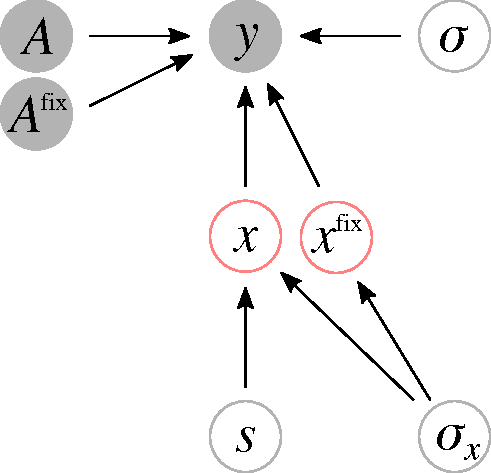
\includegraphics[width=0.25\textwidth]{figs/model-extension.pdf}
  \caption{
    \label{fig:model-extension}
    The extended model, where $A^\text{fix}$ and $x^\text{fix}$ are the feature matrix and coefficient vector for the set of features that are fixed to be active. We assume that the scale $\sigma_x$ is common the both sets of coefficients $x$ and $x^\text{fix}$.
    }
\end{figure}

We can integrate over $x$ and $x^\text{fix}$, and obtain the model evidence for $s$, as a function of $\sigma_x$ and $\alpha = \sigma/\sigma_x$,
\be
  P(y\;|\;s, \sigma_x, \alpha) = \text{Normal}(y\;|\;0, \sigma_x^2 \Phi(s,\alpha)),
\ee
where the only difference compared to \refeq{eq:nu} is the new definition of $\Phi$:
\be
  \Phi(s,\alpha) := AD_s A\T  + A^\text{fix} (A^\text{fix})\T + \alpha^2 I_M.
\ee

Similarly, we can re-define $\Psi(\tilde s)$ to
\ba
  \Psi(\tilde s) &:=& (A^\text{active}(\tilde s))\T A^\text{active}(\tilde s) + \alpha^2 I_{N_1(s)}, \qquad \text{where} \\
  A^\text{active}(\tilde s) &:=& 
  \left[\begin{array}{ccc|ccc}
  &&&&& \\
  & A^\text{fix} &&& A_{:, \tilde s} & \\
  &&&&& \\
  \end{array}\right]
\ea

\subsection{Posterior, Deployment}
\no Using the above new definition of $\Phi$ or $\Psi$, the following results apply in unchanged forms:
\begin{itemize}
  \item \refeq{eq:evidence}, and the definition of $L(s, \alpha)$,
  \item all formulas of section \ref{sec:posterior},
  \item all $\Phi$-matrix based formulas of section \ref{sec:Efficient_search}, except the maximal value of $N_{1,\text{max}}$.
  \item The intermediate variables used in the update algorithm based on $\Psi$-matrix are re-defined:
\ba
  z(\tilde s) &:=& (A^\text{active}(\tilde s))\T y \\
  B(\tilde s) &:=& (A^\text{active} (\tilde s))\T A
\ea
The formulas for $\beta_n(s)$, $G_n^\text{next}(s)$, $H_n^\text{next}(s)$ and $\ln L_n^\text{next}(s)$ are unchanged, as well as the update formula for $z, B$ and $c_k$. By computing $z$ and $B$ using their new definitions above at the beginning of the search, we are allowed to use the $\Psi$-matrix-based update algorithm in unchanged form.

\end{itemize}


Since the $A^\text{fix}$ features provide $N^\text{fix}$ new degrees of freedom that the model is trying to use to fit $y$, this lowers the maximally allowed complexity, $N_{1,\text{max}}$, from $M-2$ to:
\be
  N_{1,\text{max}} = M - 2 - N^\text{fix}.
\ee

\section{Extension: Partial pooling}
Partial pooling is a strategy to boost statistical power by  coupling inference tasks on data sets from different origin. It works if groups of data points can be regarded as ``different but not too different''. In such a case, we make use of the \emph{partial pooling} prior for the parameters in the different groups. This makes the posterior values from the different groups shrink towards a common mean. Such a correction acts as a regularization when there is little data, and with increasing evidence from the data it asymptotically vanishes, and the parameters become independent across the groups.

Here we introduce a version of the improved FBMP algorithm that uses partial pooling.

\subsection{Input data}
\no Apart from the 
\begin{itemize}
  \item feature matrix $A = \big[[a_{m,n}]_{n=1}^N\big]_{m=1}^M \in \mathds{R}^{M\times N}$ and
  \item target vector $y = [y_m]_{m=1}^M \in \mathds{R}^M$,
\end{itemize}
we assume that each sample belongs to one of $G$ groups. This information is encoded by
\begin{itemize}
  \item group indexes $g = [g_m]_{m=1}^M \in \{1,2,\ldots G\}^{\times M}$.
\end{itemize}

\subsection{Model}
The unknown linear coefficients $x = [[x_{n,g}]_{g=1}^G]_{n=1}^N \in \mathds{R}^{N\times G}$ are allowed to be different for different groups $g$. This gives rise to the following model,
\bel
  y_m = \sum_n A_{m,n} x_{n, g_m} + \varepsilon_m,
\eel
where $P(\varepsilon\;|\;\sigma) = \text{Normal}(\varepsilon\;|\; 0, \sigma^2 I_M)$, and the prior on $x_{n, g_m}$ is also normal with the following structure.
\bel
  x_{n, g} = s_n(\mu_n + d_{n, g}),
\eel
\begin{figure}[h]
\centering
  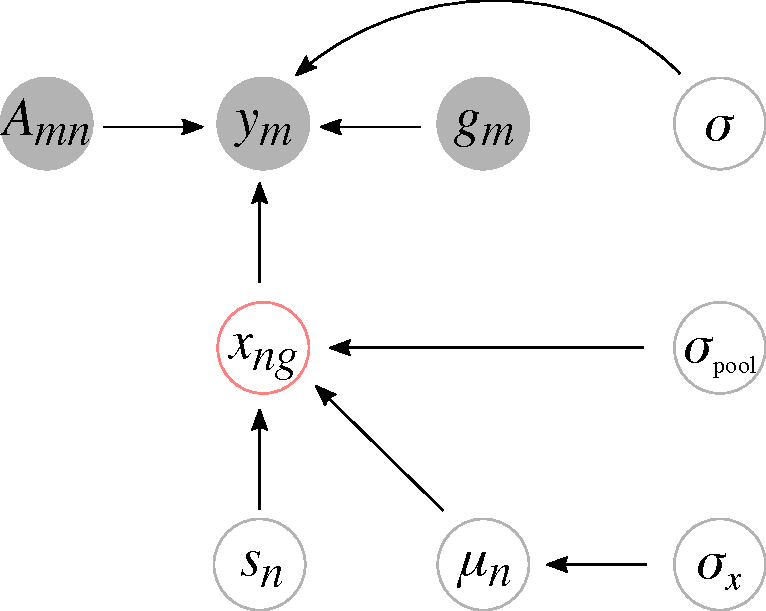
\includegraphics[width=0.4\textwidth]{figs/model-partial-pooling.pdf}
  \caption{
    \label{fig:partial-pooling}
    Partial pooling extension, where the coefficients $x_{n,g}$ are allowed to differ between groups $g$, but they are assumed to gather around the common mean $\mu_n$.
  }
\end{figure}
where the activity indicator vector $s = [s_n]_{n=1}^{N} \in \{0,1\}^{\times N}$ is independent from the group index $g$. In other words, if a feature is active in one group, it is active in all groups.
Here, $\mu_n$ is the common mean, and $d_{n, g}$ is the deviation from this mean in group $g$. We assume that they have normal priors with the following expectation values and covariances,
\ba
  \mathbb{E}(\mu_n) = 0\,\quad && \quad \text{Cov}(\mu_n, \mu_{n'}) = \sigma_x^2\delta_{n,n'}, \\
  \mathbb{E}(d_{n,g}) = 0\,\quad && \quad \text{Cov}(d_{n,g}, d_{n',g'}) = \sigma_\text{pool}^2 \delta_{n,n'}\delta_{g,g'}, \\
  && \quad \text{Cov}(\mu_n, d_{n,g}) = 0
\ea
which is equivalent to saying that all $\{\mu_n\}$ and all $\{d_{n,g}\}$ are independent from each other and have standard deviations $\sigma_x$ and $\sigma_\text{pool}$, respectively. The relative size of $\sigma_\text{pool}$ compared to $\sigma_x$ controls how similar we expect the groups to be a priori. This is the ``partial pooling'' prior. This model is depicted in \reffig{fig:partial-pooling}.



With this choice, we can compute the marginal distribution of $y$, this way, eliminating $x_{n,g}$ from the likelihood formula. The result is a normal distribution,
\be
  P(y\;|\;s, \sigma_x, \sigma, \sigma_\text{pool}) = \text{Normal}(y\;|\;0, \sigma_\text{tot}^2 \Phi(s, \alpha, \beta)),
\ee
where $\Phi$ is a function of $s$, $\alpha = \sigma / \sigma_\text{tot}$ and $\beta = \sigma_\text{pool}^2 / \sigma_\text{tot}^2$, where $\sigma_\text{tot}^2 = \sigma_x^2 + \sigma_\text{pool}^2$,
\bel
\label{eq:partial-pooling-phi}
  [\Phi(s, \alpha, \beta)]_{m,m'} = \Big((1 - \beta) + \beta \delta_{g_m, g_{m'}}\Big)\sum_{n=1}^N A_{m,n}s_nA_{m',n} + \alpha^2 \delta_{m,m'}
\eel

Using the same Inverse-Gamma prior for $\sigma_\text{tot}^2$ as before, $P(\sigma_\text{tot}^2) = \exp(-1 / \sigma_\text{tot}^2) / (\sigma_\text{tot}^2)^2$, allows us to integrate over it, yielding the following formula for the log-evidence of $s$,
\bel
  \ln P(y\;|\;s, \alpha, \beta) = \underbrace{- \frac{1}{2} \ln\det( \Phi(s,\alpha, \beta)) -\left(\frac{M}{2} + 1\right)\ln\left(1 + \frac{1}{2}y\T [\Phi(s, \alpha, \beta)]^{-1}y\right)}_{\ln L(s, \alpha, \beta)} + \text{const.}
\eel

We assume the same prior for $s$ as before, $p_s = P(s) = \intop \!d\lambda\, P(s\;|\;\lambda) P(\lambda)$, where
\ba
  P(s\;|\;\lambda) &=& \prod_{n} (1- \lambda)^{1 - s_n} (\lambda)^{s_n} \\
  P(\lambda) &=& \text{Beta}(\lambda\;|\;a = \pi \kappa, b = (1-\pi)\kappa),
\ea
which allows us to compute $p_s$ separately form $L(s,\alpha, \beta)$, and combine them to compute the empirical prior for $(\alpha, \beta)$,
\ba
  P(\alpha, \beta) \leftarrow P(\alpha, \beta\;|\;y) \approx Q_{\alpha, \beta} = \frac{p_s L(s, \alpha, \beta)}{\sum_{\alpha\in\mathcal{A}} \sum_{\beta\in\mathcal{B}} p_s L(s, \alpha, \beta)},
\ea
where $\mathcal{A}\times \mathcal{B}$ is a grid of plausible (and a priori equiprobable) values of $(\alpha, \beta)$, say $\mathcal{A} = [0.001, 0.003, 0.01, 0.03, 0.1, 0.3, 1.0, 3.0]$, and $\mathcal{B} = [0.1, 0.3, 0.5, 0.7, 0.9]$.

Using this empirical prior allows us to compute the posteriors the same way as previously, except that now we need to sum over not only $\alpha$, but $\beta$ too. E.g. the posterior activity probability of feature $n$ is
\be
  P(s_n = 1\;|\;y) \approx \frac{\sum_{\alpha \in \mathcal{A}}\sum_{\beta \in \mathcal{B}} \sum_{s:s_n=1}p_s L(s,\alpha, \beta)}{\sum_{\alpha \in \mathcal{A}}\sum_{\beta \in \mathcal{B}} \sum_{s}p_s L(s,\alpha, \beta)}.
\ee

\subsection{Efficient search of model space}
We can make use of the generalization of matrix determinant lemma and and the Woodbury matrix identity,
\ba
  \det(\Phi + UWV\T) &=& \det(\Phi)\det(W)\det(W^{-1} + V\T \Phi^{-1} U)  \\
  \Big[\Phi + UWV\T\Big]^{-1} &=& \Phi^{-1} - \Phi^{-1}U \Big(W^{-1} + V\T \Phi^{-1}U\Big)^{-1} V\T \Phi^{-1}
\ea
to compute $F(s'):=\ln \det(\Phi(s'))$ and $H(s'):=y\T \Phi(s')^{-1}y$ for a model $s'$ that differs from a ``neighboring'' $s$ in only one element, $s'_n = 1 - s_n$, using $F(s)$ and $H(s)$.
\ba
  [\Phi(s')]_{m,m'} &=& [\Phi(s)]_{m,m'} + (-1)^{s_n}(1-\beta)A_{m,n} A_{m',n} + (-1)^{s_n} \beta A_{m,n} \delta_{g_m, g_{m'}} A_{m',n} \\
  \Phi(s') &=& \Phi(s) + (-1)^{s_n}(1-\beta)a_n a_n\T + \sum_{g'=1}^G (-1)^{s_n} \beta a_n^{(g')} (a_n^{(g')})\T,
\ea
where $a_n$ is the $n$th column of the $A$ matrix, and $a_n^{(g)}$ is a projection of $a_n$ to the set of features that belong to group $g$, i.e. $[a_n^{(g')}]_m = a_n$ if $g' = g_m$ and $0$ otherwise. This represents a $G+1$-rank correction to $\Phi$.  Let's cast it into the form of $\Phi + U_n W V_n\T$, where $W$ is a $(G+1)\times (G+1)$ matrix,
\ba
  W &=& \text{diag}\Big((1-\beta), \beta, \beta, \ldots \beta\Big) \quad \in \mathds{R}^{(G+1)\times (G+1)}\\
  V_n &=& [a_n, a_n^{(1)}, a_n^{(2)}, \ldots a_n^{(G)}] \quad \in \mathds{R}^{M\times (G+1)} \\
  U_n &=& (-1)^{s_n} V_{n}.
\ea

Now, we can write the discovery and extension formulas as follows. Let's assume that we have computed the following quantities for an $s$ vector,
\ba
  F(s) &=& \ln\det(\Phi(s)) \\
  H(s) &=& y\T[\Phi(s)]^{-1}y \\
  C_k(s) &=& [\Phi(s)]^{-1} V_k.
\ea
During the ``discovery'' step we compute the following
\ba
  B_n(s) &=& \left[I_{(G+1)} + (-1)^{s_n} WV_n\T C_n(s)\right]^{-1} \\
  z_n(s) &=& C_n(s)\T y \\
  F^\text{next}_n(s) &=& F(s) - \ln\det(B_n(s)) \\
  H^\text{next}_n(s) &=& H(s) - (-1)^{s_n} z_n(s)\T WB_n(s) z_n(s) \\
  L(s') &=& -\frac{1}{2}F^\text{next}_n(s) -\left(\frac{M}{2} + 1\right) \ln\left(1 + \frac{1}{2}H^\text{next}_n(s)\right).
\ea
To close the iteration loop, we need to ``extend'' to $s'$, i.e. compute $F(s'), H(s')$ and $C_k(s')$ for all $k \in \{1,2,\ldots N\}$:
\ba
  F(s') &=& F^\text{next}_n(s) \\
  H(s') &=& H^\text{next}_n(s) \\
  C_k(s') &=& C_k(s) - (-1)^{s_n} C_n(s) \left[WB_n(s) \left(C_n(s)\T V_k\right)\right],\qquad \forall k \in \{1,2,\ldots N\}.
\ea
To further improve the efficiency of the computation, every time we need to compute $T V_k$, where $J$ is a compatible matrix, we first compute each $Ta_n^{(g')}$ for $g'\in\{1,2,\ldots G\}$, while restricting $T$ to its columns that correspond to non-zero element of $a_n^{(g')}$, and construct $TV_n$ from the results, where its first column will be $T a_n = \sum_{g'=1}^G Ta_n^{(g')}$, and all other columns are the partial results $Ta_n^{(g')}$. By doing this, we can reduce the computational complexity of this multiplication from $\mathcal{O}(M G)$ to $\mathcal{O}(M)$.

\end{document}
